\documentclass[12pt]{article}\usepackage[]{graphicx}\usepackage[]{color}
%% maxwidth is the original width if it is less than linewidth
%% otherwise use linewidth (to make sure the graphics do not exceed the margin)
\makeatletter
\def\maxwidth{ %
  \ifdim\Gin@nat@width>\linewidth
    \linewidth
  \else
    \Gin@nat@width
  \fi
}
\makeatother

\definecolor{fgcolor}{rgb}{0.345, 0.345, 0.345}
\newcommand{\hlnum}[1]{\textcolor[rgb]{0.686,0.059,0.569}{#1}}%
\newcommand{\hlstr}[1]{\textcolor[rgb]{0.192,0.494,0.8}{#1}}%
\newcommand{\hlcom}[1]{\textcolor[rgb]{0.678,0.584,0.686}{\textit{#1}}}%
\newcommand{\hlopt}[1]{\textcolor[rgb]{0,0,0}{#1}}%
\newcommand{\hlstd}[1]{\textcolor[rgb]{0.345,0.345,0.345}{#1}}%
\newcommand{\hlkwa}[1]{\textcolor[rgb]{0.161,0.373,0.58}{\textbf{#1}}}%
\newcommand{\hlkwb}[1]{\textcolor[rgb]{0.69,0.353,0.396}{#1}}%
\newcommand{\hlkwc}[1]{\textcolor[rgb]{0.333,0.667,0.333}{#1}}%
\newcommand{\hlkwd}[1]{\textcolor[rgb]{0.737,0.353,0.396}{\textbf{#1}}}%
\let\hlipl\hlkwb

\usepackage{framed}
\makeatletter
\newenvironment{kframe}{%
 \def\at@end@of@kframe{}%
 \ifinner\ifhmode%
  \def\at@end@of@kframe{\end{minipage}}%
  \begin{minipage}{\columnwidth}%
 \fi\fi%
 \def\FrameCommand##1{\hskip\@totalleftmargin \hskip-\fboxsep
 \colorbox{shadecolor}{##1}\hskip-\fboxsep
     % There is no \\@totalrightmargin, so:
     \hskip-\linewidth \hskip-\@totalleftmargin \hskip\columnwidth}%
 \MakeFramed {\advance\hsize-\width
   \@totalleftmargin\z@ \linewidth\hsize
   \@setminipage}}%
 {\par\unskip\endMakeFramed%
 \at@end@of@kframe}
\makeatother

\definecolor{shadecolor}{rgb}{.97, .97, .97}
\definecolor{messagecolor}{rgb}{0, 0, 0}
\definecolor{warningcolor}{rgb}{1, 0, 1}
\definecolor{errorcolor}{rgb}{1, 0, 0}
\newenvironment{knitrout}{}{} % an empty environment to be redefined in TeX

\usepackage{alltt}


%% packages
\usepackage{scrtime}  % for \thistime (this package MUST be listed first!)
\usepackage[margin=1in]{geometry} % page layout
\usepackage{amsmath}  % essential for cases environment
\usepackage{amsthm}   % for theorems and proofs
\usepackage{amsfonts} % mathbb
\usepackage{graphics,graphicx}
\usepackage{multirow} % fancy tables
\usepackage{wasysym}  % circle symbols (including half-filled circles)
\usepackage{enumerate}% fancier enumeration (e.g., a,b,c, ...)
%\usepackage{xcolor}
\usepackage{color}

\usepackage{amssymb,latexsym,setspace}
%%\usepackage[colorlinks,linkcolor=blue]{hyperref}
\usepackage[colorlinks=true,allcolors=blue]{hyperref}
\usepackage{xspace}
\usepackage{subfigure}
\usepackage{lineno}
\usepackage{fancyhdr}
\usepackage[english]{babel}  %% for texi2dvi ~ bug
\usepackage[normalem]{ulem}
\usepackage{tikz} % http://www.texample.net/tikz/examples/tikzdevice-demo/
  % N.B. version 0.6.3 of tikzDevice from Rforge is required!!
%% improve figure caption typsetting:  (see ~/tex/caption.pdf for manual)
\usepackage[footnotesize,bf]{caption}
\usepackage{placeins} % \FloatBarrier

%% comments
\newcommand{\de}[1]{{\color{red}{\bfseries DE:} #1}}

%% for solutions to multiple choice questions:
\newcommand{\correct}{{\color{blue}\fbox{\color{red}\checkmark} }}

%% macros
\newcommand{\reals}{\mathbb{R}}
\newcommand{\term}[1]{{\bfseries\slshape #1}}
\newcommand{\Ker}{{\text{Ker}\,}}
\newcommand{\Range}{{\text{Range}\,}}
\newcommand{\diag}{{\text{diag}}}
\newcommand{\alg}{{\text{alg}}}
\newcommand{\geom}{{\text{geom}}}
\newcommand{\norm}[1]{\left\|#1\right\|}
\newcommand{\abs}[1]{\left|#1\right|}
\newcommand{\R}{{\cal R}}
\newcommand{\G}{{\cal G}}
\newcommand{\eps}{\varepsilon}
\newcommand{\B}{\cal B}
\newcommand{\Tinf}{T_\textrm{inf}}
\newcommand{\Shat}{{\hat{S}}}
\newcommand{\Ihat}{{\hat{I}}}
\newcommand{\ie}{\emph{i.e., }}
\newcommand{\eg}{\emph{e.g., }}
\newcommand{\Rlogo}{\protect
\includegraphics[height=2ex,keepaspectratio]{../../images/Rlogo.pdf}\xspace}
\newcommand{\XPPAUT}{\texttt{XPPAUT}\xspace}
\newcommand{\etal}{\textit{et al}.\xspace}
\newcommand\emphblue[1]{\emph{\color{blue}#1}}

% citation macros
\newcommand{\citen}[1]{\cite{#1}}

% other macros
\newcommand{\avg}[1]{{\left\langle#1\right\rangle}}
\newcommand{\var}[1]{\textrm{var}\left(#1\right)}
\newcommand{\sem}[1]{\textrm{sem}\left(#1\right)}
\newcommand{\natinf}{{\mathcal I}}
\newcommand{\find}{f_{\textrm{i}}}
\newcommand{\fpop}{f_{\textrm{p}}}
\newcommand{\logit}{\textrm{logit}}
\newcommand{\sign}{\textrm{sign}}
\newcommand{\logistic}{\textrm{logistic}}
\newcommand{\code}[1]{{\tt #1}}
\newcommand{\magcode}[1]{{\tt\color{magenta}#1}}
\newcommand{\redcode}[1]{{\tt\color{red}#1}}
\newcommand{\blackcode}[1]{{\tt\color{black}#1}}

%%%%%%%%%%%%%%%%%%%
%% JOURNAL NAMES %%
%%%%%%%%%%%%%%%%%%%
\def\AJE{{\it American Journal of Epidemiology\/}}
\def\PNAS{PNAS}
\def\JAMA{JAMA}
\def\BMB{{\it Bulletin of Mathematical Biology\/}}

% references
\newcommand{\eref}[1]{Equation~\eqref{E:#1}}
\newcommand{\fref}[1]{Figure~\ref{F:#1}}
\newcommand{\tref}[1]{Table~\ref{T:#1}}
\newcommand{\sref}[1]{\S\ref{S:#1}}
% other macros
\newcommand{{\Reff}}{{\mathcal{R}}_{\rm eff}}
\newcommand{{\Sinit}}{S_{\rm init}}
\newcommand{\supp}{Supplementary Information}
\newcommand{\StoppedHere}{\bigskip\bigskip{\textcolor{red}{\hrule\centerline{\bfseries STOPPED HERE}\hrule}}\bigskip\bigskip}
\newcommand{\colvec}[2]{\begin{pmatrix}#1\\#2\end{pmatrix}}
\newcommand{\diagmat}[3]{\begin{pmatrix}#1&0&0\\0&#2&0\\0&0&#3\end{pmatrix}}

\newcommand{\solution}[1]{{\hfill\break\vspace{-0.5\baselineskip}\break\color{blue}\emph{Solution: }#1}}
\newcommand{\tr}{\text{tr}}

\newcommand{\thickredline}{\bigskip{\color{red}\hrule height 5pt}\bigskip}

%% for assignment 3:
\newtheorem{theorem}{Theorem}
\newtheorem{remark}{Remark}
\newcommand{\openset}{{\mathcal O}}
\newcommand{\C}{{\mathcal C}}

%% underline with smash through:
\newcommand*{\undersmash}[1]{\underline{\smash{#1}}}

%% referring to TeX macros
\newcommand\ttbackslash{{\tt\char`\\}}
\newcommand{\macro}[1]{{\tt\ttbackslash#1}}

%%%%%%%%%%%%%%%%%%%%%%%%%%%%%%%%%%%%%%%%%%%%%%%%%%%%%%%
%% QUESTIONS FOR MATH 4MB/6MB ASSIGNMENT 2.          %%
%% The question texts are used in several documents: %%
%% assignment, solutions, template,                  %%
%% hence it is better to load them from this file.   %%
%%%%%%%%%%%%%%%%%%%%%%%%%%%%%%%%%%%%%%%%%%%%%%%%%%%%%%%

%% \section{Plot P\&I mortality in Philadelphia in 1918}

%%% THIS WOULD BE BETTER IF IIDDA WEREN'T DOWN AT THE MOMENT:
%\item Download the data file from the International Infectious Disease Data Archive (IIDDA).  \emph{Note:} IIDDA is currently accessible only from campus or via a VPN connection.
%\begin{enumerate}[(i)]
%  \item Go to \url{http://iidda-dev.mcmaster.ca}
%  \item Request access.
%  \item After access has been granted, login and find the data file.  You can either navitage via the Mortality category or search for Philadelphia.
%\end{enumerate}

\newcommand{\PhilaDataReceived}{%
Confirm that you have received this data file by e-mail:
$$\texttt{pim\_us\_phila\_city\_1918\_dy.csv}$$
This plain text comma-separated-value file can be examined (if you wish) using any plain text editor, such as {\tt Emacs}.
}

\newcommand{\PhilaDataReadA}{%
Read the data into a data frame in \Rlogo, using the \code{read.csv()} function.  For example, the following chunk of \Rlogo code should work:
}

\newcommand{\PhilaDataReadB}{%
The purpose of the last line of code above is to ensure that \Rlogo encodes character strings such as \texttt{"1918-10-15"} as dates.
}

\newcommand{\PhilaDataReproduceA}{%
Reproduce the Philadelphia 1918 P\&I plot:
}

\newcommand{\PhilaDataReproduceB}{%
You'll need to use functions such as \code{plot()}, \code{points()} and \code{lines()}.  For a comprehensive list of graphics parameters accepted by these functions, enter {\tt ?par} into the Console pane in {\tt RStudio}.  There are multiple ways to produce a graph exactly like the above, but the following steps work:
\begin{itemize}
  \item Use \code{plot()} to draw the box and basic annotation and the grey line.  Suppress labels when doing this (\emph{e.g.,} \code{xlab=""}).  The box type is controlled by the \code{bty} option and the orientation of annotation is controlled by the \code{las} option.
  \item Use \code{points()} to draw the heavy red dots with black borders.  The most elegant way to do this is to set the point character type to 21 (\code{pch=21}) and the point background colour to red (\code{bg="red"}).  Alternatively, you can use \code{points()} twice (first to draw the red dots and then to draw the black circles around them).
  \item Use \code{mtext()} to add the $x$ and $y$ axis labels in the margins of the plot.
\end{itemize}
}

%% \section{Estimate $\R_0$ from the Philadelphia P\&I time series}

\newcommand{\EstimateRna}{%
The observed mortality time series $M(t)$ is certainly not equal to the prevalence $I(t)$ that appears in the SIR model.  Suppose, however, that $I(t) = \eta M(t-\tau)$ for all time (where $\eta$ and $\tau$ are constants), \emph{i.e.,} that the mortality curve is exactly a scaled and translated version of the prevalence curve.  Prove that if both $I$ and $M$ are growing exactly exponentially over some time period then their exponential rates are identical.  Thus, if we compare them during the ``exponential phase'' on a logarithmic scale, then both curves will be perfectly straight with exactly the same slope.
}

\newcommand{\EstimateRnb}{%
Fit a straight line to the part of the Philadelphia 1918 mortality time series that looks straight on a logarithmic scale (and show your result in a plot).  Once you get the hang of it, the easiest way to do this is to use the \code{lm()} function in \Rlogo (lm stands for linear model).  Note that the simplest way to draw a straight line with given slope and intercept is with the \code{abline()} function.  If you find \code{lm()} counter-intutive to understand then experiment with \code{abline()} until your eyes tell you that you have discovered a line that provides a good fit.
}

\newcommand{\EstimateRnc}{%
How is the slope of your fitted line related to the parameters of the SIR model?  (\emph{Hint:} When $I$ is small, $S\simeq1$.) Why do you need an independent measure of the mean infectious period to estimate $\R_0$?  If the mean infectious period is 4 days, what is your estimate of $\R_0$?
}

%% \section{Fit the basic SIR model to the Philadelphia P\&I time series}

\newcommand{\FitSIRa}{%
Install the \code{"deSolve"} package.  This
    is done by typing the following command in the Console pane of
    {\tt RStudio}:
    $$\text{\code{install.packages("deSolve")}}$$
You will then be prompted to choose a mirror site from which to download the package.  It doesn't matter which mirror you choose, but choosing a site in Ontario might save a fraction of a second. \emph{Note:} This is a one-time operation.  You do not want an \code{install.packages()} command inside your solutions code.
}

\newcommand{\FitSIRbIntro}{%
Write an \Rlogo function that plots the solution $I(t)$ of the SIR model for given parameter values ($\R_0$ and $1/\gamma$) and given initial conditions ($S_0,I_0$).  Use the {\tt ode()} function in the {\tt deSolve} package.
}

\newcommand{\FitSIRbii}{%
As an example of defining a function (without getting involved with a differential equation), here is a code chunk that defines a function to plot a sine curve, and then executes the function.  Note that the default min and max $x$ values are set in the parameter list of the function definition, but the max $x$ value is changed when the function is executed:
}

\long\def\FitSIRbiiiA{%
Here's another example.  This time we first define the vector field for a differential equation.  We then use this function inside another function that plots the solution of the associated differential equation.  To understand the construction, you can, as usual, study the help page for the calling function (\code{?ode} in this case), but the most important issues are the following.

One of the arguments of the \code{ode()} function is the function that evaluates the vector field at the current time.  To avoid confusion, choose the arguments of your vector field function to be \code{t}, \code{vars} and \code{parms} (in that order):
\begin{center}
\begin{tabular}{r p{4.25in}}
     \code{t} & The current time, which will be used within the vector field function if the system is non-autonomous. \\
     \code{vars} & A named vector of the variables in the system (\eg $S$, $I$).  The variables, as named vector passed to this function, are used in the code that defines the vector field within the function. \\
     \code{parms} & A named vector of the parameters of the system (\eg $\beta$, $\gamma$).  It is convenient---but not necessary---to specify default values for the parameters.
\end{tabular}
\end{center}

It is strongly recommended that you follow exactly the style below when defining vector fields for differential equations that you wish to solve with the \code{ode()} function.  In particular, the construction ``\code{with(as.list(c(parms,vars)), {...})}'' makes the variables and parameters visible within the section of code between the braces (\code{\{...\}}) without having to refer to the vectors or lists in which they are stored.  For example, the code would be much harder to read if each instance of \code{x} were replaced by \code{vars\$x} and each instance of \code{beta} were replaced by \code{parms\$beta}; this issue becomes extremely important for complicated vector fields.
}

\newcommand{\FitSIRbiiiB}{%
The following function plots a single solution of the ODE for a given initial condition (\code{ic}), integration time (\code{tmax}) and times at which the state is to be returned (\code{times}).  The vector field function is passed as the \code{func} argument and the parameter vector is passed as the \code{parms} argument.  If further arguments are given, they are passed to the \code{lines()} function that draws the solution.
}

\newcommand{\FitSIRbiiiC}{%
Note here that the call to the \code{ode()} function gives the arguments in the default order so they are interpretted correctly.  If we wished to write the arguments in a different order then we would have to be explicit about which argument is which.  For example, if we wanted to list the initial conditions last for some deep reason then we would have to write:
}

\newcommand{\FitSIRc}{%
For $I_0=10^{-3}$ and $S_0=1-I_0$, plot the solutions of the SIR model assuming $1/\gamma=4$ days and $\R_0\in\{1.2,1.5,1.8,2,3,4\}$.  Use the \code{legend()} command to make a legend on the plot that shows which curves correspond to which values of $\R_0$.
}

\newcommand{\FitSIRd}{%
By trial and error, find values of $\R_0$ and $\gamma$ that yield a solution of the SIR model that fits the Philadelphia P\&I times series reasonably well.  You can assess the quality of fit using the Euclidean distance between the model solution and the data.  (\emph{Note:}  The trial and error approach is a valuable exercise, but not a suggestion of a method you would really use in practice.  We'll discuss better methods for fitting ODE models to data later.)
}

%% \section{Executive summary for the Public Health Agency}

\long\def\ExecSumm{%
The Public Health Agency of Canada (PHAC) is revising their pandemic plan and has asked your group to summarize what you learned from analyzing the 1918 Philadelphia P\&I time series.  Besides explaining what inferences you feel you can make from your analysis so far, PHAC wants to know what you would investigate if they were to fund you to continue your work full time for a month.  They want a maximum of one page from your group.

Incidentally, you might be interested to know that rumour has it that all of the members of the pandemic planning committee took Math 2C03 at McMaster University between 1980 and 2003, but they all failed.  Also, when the chair of the committee was recently asked ``What is a differential equation?'' he apparently bent over and vomited (it is hard to know quite what to make of this given that PHAC was investigating a norovirus outbreak at the time).

\smallskip
\noindent{\em\underline{Note}: When submitting your assignment solution, it is imperative that the one-page executive summary be printed on its own page.  To start a new page in \LaTeX, use the \macro{newpage} command.  Also, as usual, your summary should be in 12 point font.  Don't try to cram in as much as possible.  Make that page as clear and concise as you can, so that a public health planner can absorb its content quickly and easily.}
}

%%\bibliographystyle{vancouver}
%%\bibliography{4mba2_2018}


%%%%%%%%%%%%%%%%%%%%%%%%%%%%%%%%%%%
%% FANCY HEADER AND FOOTER STUFF %%
%%%%%%%%%%%%%%%%%%%%%%%%%%%%%%%%%%%
\usepackage{fancyhdr,lastpage}
\pagestyle{fancy}
\fancyhf{} % clear all header and footer parameters
%%%\lhead{Student Name: \theblank{4cm}}
%%%\chead{}
%%%\rhead{Student Number: \theblank{3cm}}
%%%\lfoot{\small\bfseries\ifnum\thepage<\pageref{LastPage}{CONTINUED\\on next page}\else{LAST PAGE}\fi}
\lfoot{}
\cfoot{{\small\bfseries Page \thepage\ of \pageref{LastPage}}}
\rfoot{}
\renewcommand\headrulewidth{0pt} % Removes funny header line
%%%%%%%%%%%%%%%%%%%%%%%%%%%%%%%%%%%
\IfFileExists{upquote.sty}{\usepackage{upquote}}{}
\begin{document}

\begin{center}
{\bf Mathematics 4MB3/6MB3 Mathematical Biology\\
\smallskip
\url{http://www.math.mcmaster.ca/earn/4MB3}\\
\smallskip
2019 ASSIGNMENT 2}\\
\medskip
\underline{\emph{Group Name}}: \texttt{{\color{blue}Cream}}\\
\medskip
\underline{\emph{Group Members}}: {\color{blue}Eric Clapton, Ginger Baker, Jack Bruce}
\end{center}

\bigskip
\noindent
This assignment was due in class on \textcolor{red}{\bf Monday 4 February 2019 at 9:30am}.

\section{Plot P\&I mortality in Philadelphia in 1918}

\begin{enumerate}[(a)]

\item \PhilaDataReceived

\item \PhilaDataReadA
\begin{knitrout}
\definecolor{shadecolor}{rgb}{0.969, 0.969, 0.969}\color{fgcolor}\begin{kframe}
\begin{alltt}
\hlstd{datafile} \hlkwb{<-} \hlstr{"pim_us_phila_city_1918_dy.csv"}
\hlstd{philadata} \hlkwb{<-} \hlkwd{read.csv}\hlstd{(datafile)}
\hlstd{philadata}\hlopt{$}\hlstd{date} \hlkwb{<-} \hlkwd{as.Date}\hlstd{(philadata}\hlopt{$}\hlstd{date)}
\end{alltt}
\end{kframe}
\end{knitrout}
\PhilaDataReadB

\item \PhilaDataReproduceA

  {\color{blue} \begin{proof}[Solution]
  {\color{magenta}\dots beautiful graph here\dots\ and nicely commented code that produces it, either in a separate \texttt{.R} file or preceding the graph if this is a \texttt{knitr} script\dots}
  \end{proof}
  }

\PhilaDataReproduceB

\end{enumerate}

\section{Estimate $\R_0$ from the Philadelphia P\&I time series}

\begin{enumerate}[(a)]

\item \EstimateRna

 {\color{blue} \begin{proof}[Solution]
 {\color{magenta}\dots beautifully clear and concise text to be inserted here\dots}
 \end{proof}
 }

\item \EstimateRnb

  {\color{blue} \begin{proof}[Solution]
  {\color{magenta}\dots beautifully clear text and plot(s) here \dots\ interspersed with \Rlogo code if this is a \texttt{knitr} script}
  \end{proof}
  }

\item \EstimateRnc

  {\color{blue} \begin{proof}[Solution]
  {\color{magenta}\dots beautifully clear text here \dots\ including some embedded \Rlogo code to estimate $\R_0$ if this is a \texttt{knitr} script}
  \end{proof}
  }

\end{enumerate}

\section{Fit the basic SIR model to the Philadelphia P\&I time series}

\begin{enumerate}[(a)]

\item \FitSIRa

\item \FitSIRbIntro
\begin{itemize}
    \item Your code will first need to load the \code{deSolve} package:
\begin{knitrout}
\definecolor{shadecolor}{rgb}{0.969, 0.969, 0.969}\color{fgcolor}\begin{kframe}
\begin{alltt}
\hlkwd{library}\hlstd{(}\hlstr{"deSolve"}\hlstd{)}
\end{alltt}


{\ttfamily\noindent\bfseries\color{errorcolor}{\#\# Error in library("{}deSolve"{}): there is no package called 'deSolve'}}\end{kframe}
\end{knitrout}
    \item \FitSIRbii
\begin{knitrout}
\definecolor{shadecolor}{rgb}{0.969, 0.969, 0.969}\color{fgcolor}\begin{kframe}
\begin{alltt}
\hlstd{plot.sine} \hlkwb{<-} \hlkwa{function}\hlstd{(} \hlkwc{xmin}\hlstd{=}\hlnum{0}\hlstd{,} \hlkwc{xmax}\hlstd{=}\hlnum{2}\hlopt{*}\hlstd{pi ) \{}
  \hlstd{x} \hlkwb{<-} \hlkwd{seq}\hlstd{(xmin,xmax,}\hlkwc{length}\hlstd{=}\hlnum{100}\hlstd{)}
  \hlkwd{plot}\hlstd{(x,} \hlkwd{sin}\hlstd{(x),} \hlkwc{typ}\hlstd{=}\hlstr{"l"}\hlstd{)}
  \hlkwd{grid}\hlstd{()} \hlcom{# add a light grey grid}
\hlstd{\}}
\hlkwd{plot.sine}\hlstd{(}\hlkwc{xmax}\hlstd{=}\hlnum{4}\hlopt{*}\hlstd{pi)}
\end{alltt}
\end{kframe}
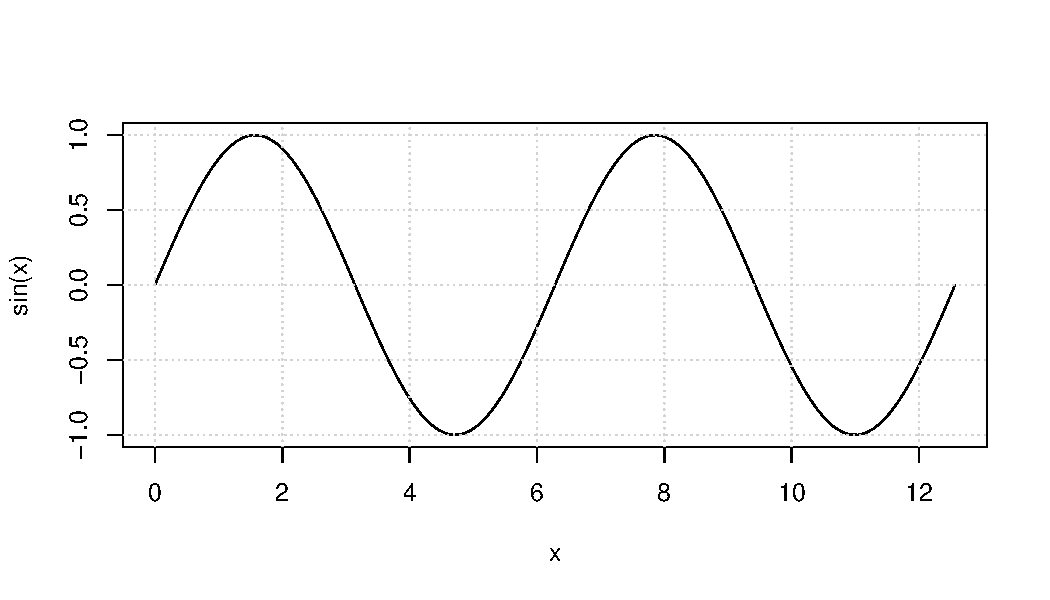
\includegraphics[width=\maxwidth]{figure/plot_sine-1} 

\end{knitrout}
  \item \FitSIRbiiiA
\begin{knitrout}
\definecolor{shadecolor}{rgb}{0.969, 0.969, 0.969}\color{fgcolor}\begin{kframe}
\begin{alltt}
\hlcom{## Vector Field for SI model}
\hlstd{SI.vector.field} \hlkwb{<-} \hlkwa{function}\hlstd{(}\hlkwc{t}\hlstd{,} \hlkwc{vars}\hlstd{,} \hlkwc{parms}\hlstd{=}\hlkwd{c}\hlstd{(}\hlkwc{beta}\hlstd{=}\hlnum{2}\hlstd{,}\hlkwc{gamma}\hlstd{=}\hlnum{1}\hlstd{)) \{}
  \hlkwd{with}\hlstd{(}\hlkwd{as.list}\hlstd{(}\hlkwd{c}\hlstd{(parms, vars)), \{}
    \hlstd{dx} \hlkwb{<-} \hlopt{-}\hlstd{beta}\hlopt{*}\hlstd{x}\hlopt{*}\hlstd{y} \hlcom{# dS/dt}
    \hlstd{dy} \hlkwb{<-} \hlstd{beta}\hlopt{*}\hlstd{x}\hlopt{*}\hlstd{y}  \hlcom{# dI/dt}
    \hlstd{vec.fld} \hlkwb{<-} \hlkwd{c}\hlstd{(}\hlkwc{dx}\hlstd{=dx,} \hlkwc{dy}\hlstd{=dy)}
    \hlkwd{return}\hlstd{(}\hlkwd{list}\hlstd{(vec.fld))} \hlcom{# ode() requires a list}
  \hlstd{\})}
\hlstd{\}}
\end{alltt}
\end{kframe}
\end{knitrout}

\FitSIRbiiiB
\begin{knitrout}
\definecolor{shadecolor}{rgb}{0.969, 0.969, 0.969}\color{fgcolor}\begin{kframe}
\begin{alltt}
\hlcom{## Draw solution}
\hlstd{draw.soln} \hlkwb{<-} \hlkwa{function}\hlstd{(}\hlkwc{ic}\hlstd{=}\hlkwd{c}\hlstd{(}\hlkwc{x}\hlstd{=}\hlnum{1}\hlstd{,}\hlkwc{y}\hlstd{=}\hlnum{0}\hlstd{),} \hlkwc{tmax}\hlstd{=}\hlnum{1}\hlstd{,}
                      \hlkwc{times}\hlstd{=}\hlkwd{seq}\hlstd{(}\hlnum{0}\hlstd{,tmax,}\hlkwc{by}\hlstd{=tmax}\hlopt{/}\hlnum{500}\hlstd{),}
                      \hlkwc{func}\hlstd{,} \hlkwc{parms}\hlstd{,} \hlkwc{...} \hlstd{) \{}
  \hlstd{soln} \hlkwb{<-} \hlkwd{ode}\hlstd{(ic, times, func, parms)}
  \hlkwd{lines}\hlstd{(times, soln[,}\hlstr{"y"}\hlstd{],} \hlkwc{col}\hlstd{=}\hlstr{"blue"}\hlstd{,} \hlkwc{lwd}\hlstd{=}\hlnum{3}\hlstd{, ... )}
\hlstd{\}}
\end{alltt}
\end{kframe}
\end{knitrout}
\FitSIRbiiiC
\begin{knitrout}
\definecolor{shadecolor}{rgb}{0.969, 0.969, 0.969}\color{fgcolor}\begin{kframe}
\begin{alltt}
  \hlstd{soln} \hlkwb{<-} \hlkwd{ode}\hlstd{(}\hlkwc{times}\hlstd{=times,} \hlkwc{func}\hlstd{=func,} \hlkwc{parms}\hlstd{=parms,} \hlkwc{y}\hlstd{=ic)}
\end{alltt}
\end{kframe}
\end{knitrout}

We can now use our \code{draw.soln()} function to plot a few solutions of the SI model.

\begin{knitrout}
\definecolor{shadecolor}{rgb}{0.969, 0.969, 0.969}\color{fgcolor}\begin{kframe}
\begin{alltt}
\hlcom{## Plot solutions of the SI model}
\hlstd{tmax} \hlkwb{<-} \hlnum{10} \hlcom{# end time for numerical integration of the ODE}
\hlcom{## draw box for plot:}
\hlkwd{plot}\hlstd{(}\hlnum{0}\hlstd{,}\hlnum{0}\hlstd{,}\hlkwc{xlim}\hlstd{=}\hlkwd{c}\hlstd{(}\hlnum{0}\hlstd{,tmax),}\hlkwc{ylim}\hlstd{=}\hlkwd{c}\hlstd{(}\hlnum{0}\hlstd{,}\hlnum{1}\hlstd{),}
     \hlkwc{type}\hlstd{=}\hlstr{"n"}\hlstd{,}\hlkwc{xlab}\hlstd{=}\hlstr{"Time (t)"}\hlstd{,}\hlkwc{ylab}\hlstd{=}\hlstr{"Prevalence (I)"}\hlstd{,}\hlkwc{las}\hlstd{=}\hlnum{1}\hlstd{)}
\end{alltt}
\end{kframe}
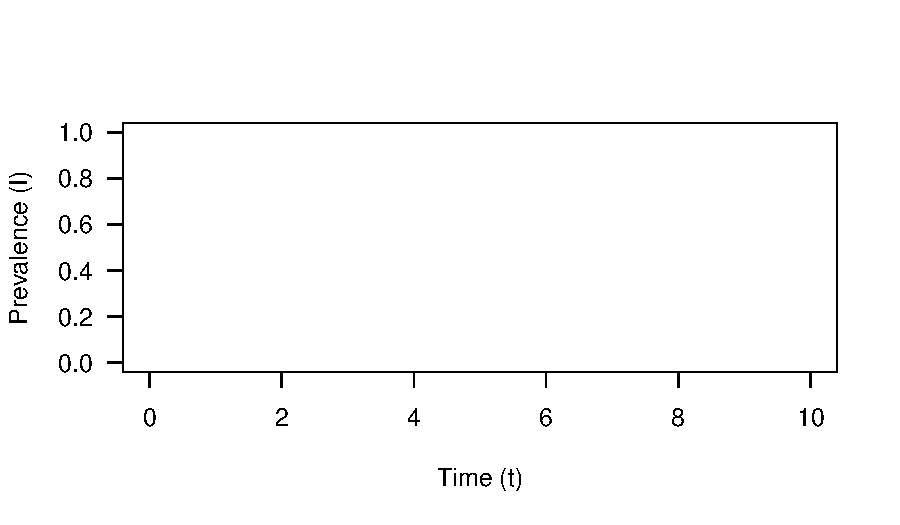
\includegraphics[width=\maxwidth]{figure/plot_SI_model-1} 
\begin{kframe}\begin{alltt}
\hlcom{## initial conditions:}
\hlstd{I0} \hlkwb{<-} \hlnum{0.001}
\hlstd{S0} \hlkwb{<-} \hlnum{1} \hlopt{-} \hlstd{I0}
\hlcom{## draw solutions for several values of parameter beta:}
\hlstd{betavals} \hlkwb{<-} \hlkwd{c}\hlstd{(}\hlnum{1.5}\hlstd{,}\hlnum{2}\hlstd{,}\hlnum{2.5}\hlstd{)}
\hlkwa{for} \hlstd{(i} \hlkwa{in} \hlnum{1}\hlopt{:}\hlkwd{length}\hlstd{(betavals)) \{}
  \hlkwd{draw.soln}\hlstd{(}\hlkwc{ic}\hlstd{=}\hlkwd{c}\hlstd{(}\hlkwc{x}\hlstd{=S0,}\hlkwc{y}\hlstd{=I0),} \hlkwc{tmax}\hlstd{=tmax,}
            \hlkwc{func}\hlstd{=SI.vector.field,}
            \hlkwc{parms}\hlstd{=}\hlkwd{c}\hlstd{(}\hlkwc{beta}\hlstd{=betavals[i],}\hlkwc{gamma}\hlstd{=}\hlnum{1}\hlstd{),}
            \hlkwc{lty}\hlstd{=i} \hlcom{# use a different line style for each solution}
            \hlstd{)}
\hlstd{\}}
\end{alltt}


{\ttfamily\noindent\bfseries\color{errorcolor}{\#\# Error in ode(ic, times, func, parms): could not find function "{}ode"{}}}\end{kframe}
\end{knitrout}


  \end{itemize}

 {\color{blue} \begin{proof}[Solution]
 {\color{magenta}\dots If this is a \texttt{knitr} script then your code should be displayed here.  Otherwise, you should state here the name of the file where the \Rlogo code is, and the names of any functions you defined\dots}
 \end{proof}
 }

\item \FitSIRc

  {\color{blue} \begin{proof}[Solution]
  {\color{magenta}\dots beautifully clear text and plot(s) here \dots\ preceded by \Rlogo code if this is a \texttt{knitr} script}
  \end{proof}
  }

\item \FitSIRd

  {\color{blue} \begin{proof}[Solution]
  {\color{magenta}\dots beautifully clear text and plot(s) here \dots\ interspersed with \Rlogo code if this is a \texttt{knitr} script}
  \end{proof}
  }

\end{enumerate}

\section{Executive summary for the Public Health Agency}

\ExecSumm

  {\color{blue} \begin{proof}[Solution]
  {\color{magenta}\dots beautifully clear executive summary here, on its own page\dots}
  \end{proof}
  }

\bigskip

\centerline{\bf--- END OF ASSIGNMENT ---}

\bigskip
Compile time for this document:
\today\ @ \thistime

\end{document}
